\documentclass[12pt]{article}
\usepackage{titling}
\usepackage{graphicx}

\setlength{\parindent}{0in}
\setlength{\parskip}{10pt}

\usepackage[margin=1in]{geometry}

\title{Life Tracker Version 2.0 Functional and Technical Specifications}
\author{Stuart Larsen \ \  Carl Vitullo}
\date{\today}

\begin{document}
\maketitle
\thispagestyle{empty}

\pagebreak
\thispagestyle{empty}
\tableofcontents
\thispagestyle{empty}
\clearpage

\section{Overview}

LifeTracker is a service that helps people do temporal analysis on events in their life.

Users can mark events on a timeline, such as ``Woke Up'', ``Doing Homework'', ``Took Medicine''. After a few events over a few days have been recorded, analysis can be done on the data.

The service will show you how frequent events occur, how long events last (if they are duration events, more on that later), and the relationships between other events. The idea is to find relationship between things in your life that you didn't even know.

\section{Scenarios}

The following subsections will outline how a few different users can approach this service in a benificial manner.

\subsection{College Student Mike}

College Student Mike hasen't been doing so well in his classes. He just never seems to have enough time to his homework or study for exams. Where does all of his time go?

Mike starts an account at LifeTracker and begins recording all the events he does in his life. After maybe a weke of this, he can see exactly where all his time went.

\begin{figure}[h!]
  \centering
  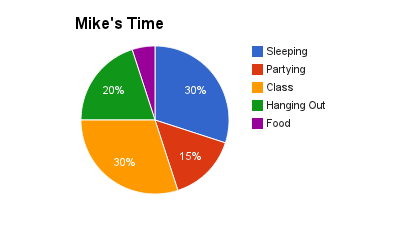
\includegraphics[scale=.9]{images/mikeChart}
  \caption{How Mike Spends His Time}
  \label{fig:mikeChart}
\end{figure}

From the graph you can see the reason he is failing his classes is because he spends 15\% of his time partying, and 20\% of his time Hanging Out, but no time doing homework or studying.

\subsection{Sad Day Steve}

Steve has been feeling very sad lately. Steve thinks it's because of his sleep schedule, but he doesn't really know.

So Steve creates an account at LifeTracker. He records the time he goes to bed each night, and the time he wakes up each morning. And everyday he reccords his mood.

After a few weeks of reccording, he discovers the following relationship:

\begin{figure}[h!]
  \centering
  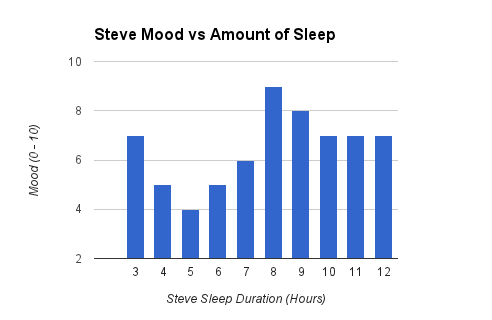
\includegraphics[scale=.9]{images/steveChart}
  \caption{Steves Mood per Hours of Sleep}
  \label{fig:steveChart}
\end{figure}

Steve now knows that he is on average in the best mood when he sleeps 8ish hours. It's also interesting to note that he feels a lot better after 3 hours of sleep compared to 4 hours of sleep.

\section{Functional Specifications}

\begin{figure}[h!]
  \centering
  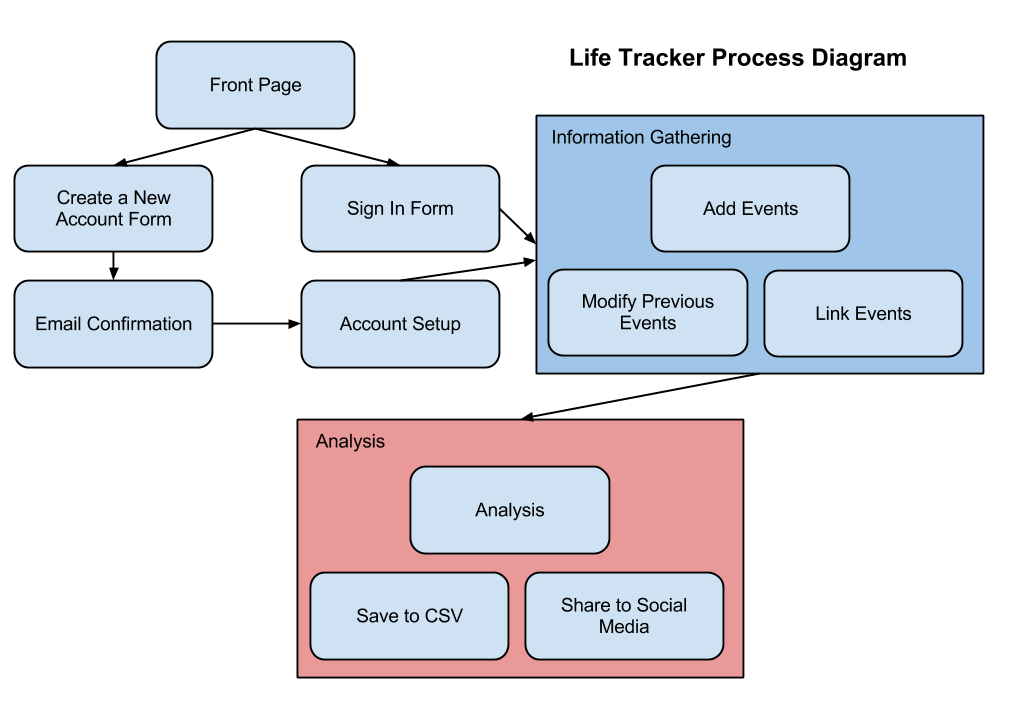
\includegraphics[scale=.5]{images/procDiag}
  \caption{LifeTracker Process Diagram}
  \label{fig:procDiag}
\end{figure}

\subsection{Front Page}

The front page is the entry point into the program. If a user is already logged in, it will redirect to home.html. Otherwise it will contain the following:

\begin{itemize}
  \item Short Description of what LifeTracker is
  \item Login on Top Right
  \item Create New Account Link
  \item ``Slide Show'' of various graphs and charts, with little quotes, testimonials in center frame
\end{itemize}

\subsection{Sign In Form}

A simple login form, email and password. There will be two passwords and email fields for simple spell checking validation.

\begin{itemize}
  \item Form for email and password
  \item \textit{Forget Password?} Link
\end{itemize}

\subsubsection{Possible Failure Cases}
\begin{description}
  \item[Failed Multiple Attempts] \hfill \\
    Lock account for 15 minutes after 5 failed attempts. Send email to user notifying failed attempts.
  \item[Forgot Password] \hfill \\
    Enter just the email and a reset password will be sent.
\end{description}

\subsubsection{Future Ideas}
\begin{itemize}
  \item Use google login or facebook login
\end{itemize}

\subsection{Create a New Account Form}

User enters in the following information:
\begin{itemize}
  \item Name
  \item email twice
  \item password twice
\end{itemize}

Each input field should have a validators on the front end.

\subsubsection{Possible Failure Cases}
\begin{description}
  \item[Email Already in Use] \hfill \\
    Help retrieve password
\end{description}

\subsection{Information Gathering}

During this stage the user can click an Add Event button which will pop up a form asking the user for information on the event, such as: Name/Label, Time of Event, Description, and ask if they want to link it with another event.

For Version 1.0 this information will be stored into a table on the main page.

There will be links to analysis and logout on the top.

\subsubsection{Notes}

I think event adding with really need to be streamlined. It needs to be as easy as possible to add new events. Information is power.

\subsection{Analysis}

On this page there will be graphs and charts showing relationships between the various forms of information. 

\subsubsection{Possible Analysis Views}

\begin{description}
  \item[Time Spent Per Label] \hfill \\
    Pie Chart, shows how time is divied up per label
  \item[Number of Occurrences Per Label Per Day] \hfill \\
    Histogram, shows how often each event happens per day
  \item[Averages] \hfill \\
    Table, gives each label, and the average time of occurrance, how many times it occurs, on average how many times it occurrs. 
\end{description}

\subsubsection{Notes}

I think once everything is set up, this'll be the hardest part. This NEEDs to be well thought out and as modular as possible.

\section{Technical Specifications}

\subsection{Django}

The backend framework will be Django. 

\subsubsection{Views}

\begin{enumerate}
  \item Home Page
  \item Login
  \item New Account
  \item Main Page
  \item Add Event
  \item Analytics
\end{enumerate}

\subsubsection{Models}

\begin{description}
  \item[Events] \hfill \\
    Each item added to the timeline is an event. Events contain a label, such as ``Sleeping'', a datetime stamp, a small description, and links. Events can be linked together to show duration of events, or occurances, such as ``taking medicine''.
 \item[Label] \hfill \\
  Labels are the strings that describe events. Such as ``Going to Sleep''. They show similarities between events.
 \item[User] \hfill \\
   Each user has their own set of labels and events. Along with email name password and such.
\end{description}

\section{Future}

\subsection{Mood}

Tracks events and ties mood to each event. Mood updates can also be events.

But I imagine two time charts, one for events and one for moods:

\begin{verbatim}
Events:
Woke Up    Lunch   Off Work         Sleep
|          |         |               |
-----------------------------------------

Mood:
  -        ---        ---   ---------
 - ---------  -      -   - -
-              ------     -

\end{verbatim}

So users can see how events in their life effects thier mood. There will be a rating scale from 0-10 on how ``happy'' they are. They can either submit a numebr from 0-10 or, say there was an increase of happiness from when they last said they were happy.

\end{document}
